\chapter{PROFIL INSTITUSI KERJA PRAKTEK}
\section{Merdeka Belajar - Kampus Merdeka}
\begin{figure}[H]
	\centering
	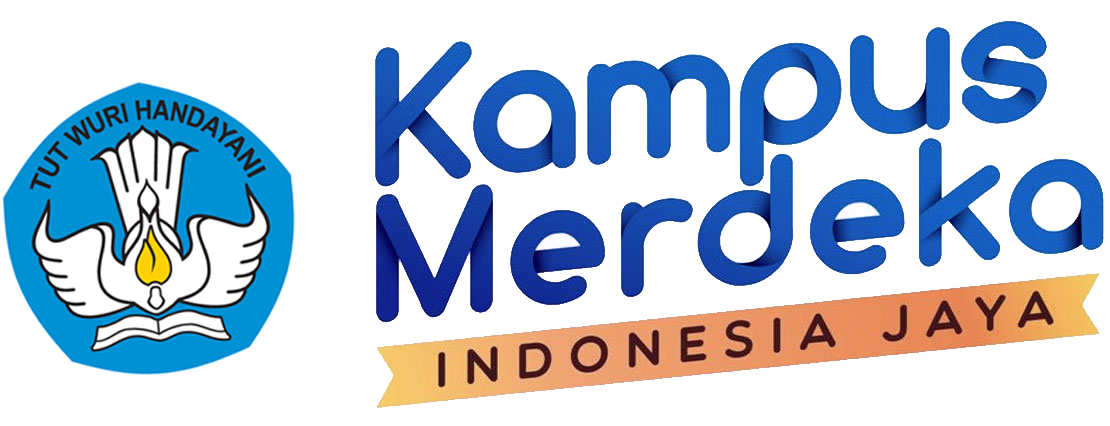
\includegraphics[scale=0.25]{./assets/logombkm}
	\caption{Logo Kampus Merdeka.}
\end{figure}
Merdeka Belajar - Kampus Merdeka merupakan kebijakan Menteri Pendidikan dan Kebudayaan yang bertujuan mendorong mahasiswa untuk menguasai berbagai keilmuan yang berguna untuk memasuki dunia kerja. Kebijakan Kampus Merdeka ini sesuai dengan Permendikbud Nomor 3 Tahun 2020 tentang Standar Nasional Pendidikan Tinggi, dan diluncurkan pada Januari 2020.

Melalui program Kampus Merdeka, mahasiswa memiliki kesempatan satu semester atau setara dua puluh SKS untuk menempuh pembelajaran luar program studi pada Perguruan Tinggi yang sama. Terdapat beberapa program dari Kampus Merdeka, seperti Magang, Studi Independen, Bangkit Academy, Indonesia International Student Mobility Awards (IISMA), Kampus Mengajar, GERILYA ESDM, KKN Tematik, Pejuang Muda Kampus Merdeka, Pertukaran Mahasiswa Merdeka, Proyek Kemanusiaan, Riset, dan Wirausaha.

Pendaftaran program Kampus Merdeka biasanya dibuka pada awal dan pertengahan tahun, seiring dengan bermulainya perkuliahan semester genap dan ganjil. Pada periode ini, penulis bergabung mengikuti program Bangkit Academy.

\section{Bangkit Academy}
\begin{figure}[H]
	\centering
	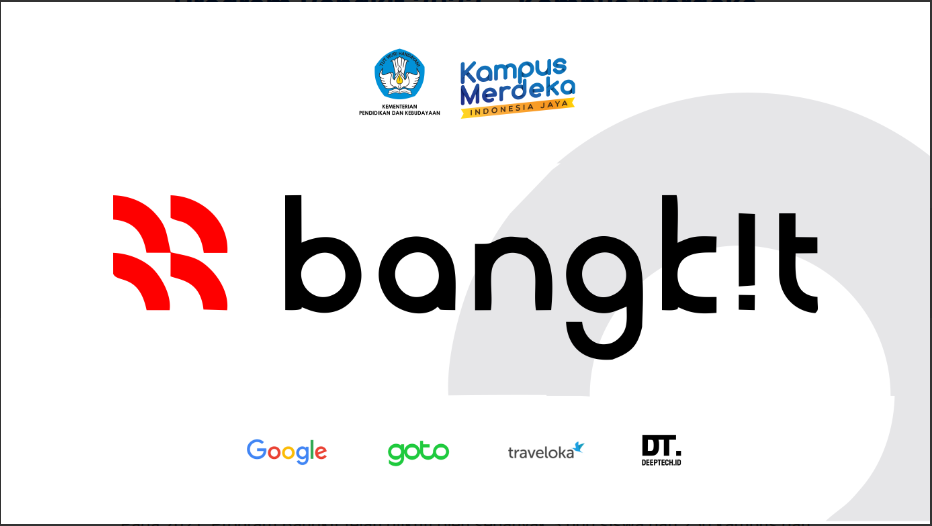
\includegraphics[scale=0.25]{./assets/logobangkit}
	\caption{Logo Bangkit Academy 2022.}
\end{figure}
Sebagai kerjasama antara Google, GoTo, Traveloka, Kemendikbudristek, dan beragam Perguruan Tinggi di Indonesia, Bangkit Academy adalah sebuah program studi independen yang merupakan bagian dari Kampus Merdeka. Pada program Bangkit, lebih dari 3000 mahasiswa terpilih dibagi dalam 3 \textit{learning path}, yakni \textit{Cloud Computing, Machine Learning}, dan \textit{Android Develpment}. Program Bangkit dilaksanakan dari tanggal 14 Februari 2022 sampai dengan 27 Juli 2022.

Selain kursus mengenai IT yang telah disebutkan, Bangkit juga memberikan kuliah mengenai \textit{Soft Skills} yang mempersiapkan mahasiswa untuk terjun ke dunia kerja, memberikan wawasan cara bekerjanya sebuah perusahaan berbasis IT, mengajarkan mahasiswa cara berwirausaha, cara berkomunikasi, dan cara membangun sebuah \textit{branding} bagi pribadi mahasiswa.